  \maketitle
  \pnote{
      Thank you very much Prof. Rückert for the kind introduction.\\
      Thanks to my committee for examining my work\\
      and to everyone else for participating in my defence.\\
      Welcome to my defence with the title: \\
  }
\begin{frame}{Interaction in Smart Environments - the CSRA}
  \begin{columns}[T] % align columns
    \begin{column}{.65\textwidth}
    \centering
    \resizebox{1.\textwidth}{!}{%
        \footnotesize
        \begin{tikzpicture}
        \action<1->{\node (a) at (0,0)
        {
          \resizebox{\textwidth}{!}{%
            
\includegraphics[width=\textwidth]{generated/csra-shots.pdf}
          }
        };}
      \end{tikzpicture}
    }
    \end{column}%
    \begin{column}{.4\textwidth}
      \vspace{20pt}
      \centering
        Devices, Agents \& Robot \\
      \vspace{5pt}
        24/7\\
        \pause
        \textcolor{myred}{\faArrowDown}\\
        Addressing\\
        Attention\\
        Civil inattention
    \end{column}%
    \end{columns}
    \pnote{
      45-40 - CSRA\\
      Full of interactive devices agents robots\\
      Flobis left, floka center\\
      Operational 24/7\\
      person enters (click) entities have to know\\
      what happens when they do not know? \\
      }
\end{frame}
\begin{frame}[standout]
  \centering
  \pdfpcmovie[width=.98\textwidth]{\includegraphics[width=.98\textwidth]{generated/elevator.jpg}}{generated/elevator.mp4}
  \\\tiny{Elevator scene \url{https://www.youtube.com/watch?v=BgRoiTWkBHU}}\\
  \pnote{
    45-40 - short video of an elevator\\
    guy with tie center of interest\\
    others are actors, oriented towards backside of elevator\\
    yout may know but lets look what happens to the guy (click)\\
    agents in out copresense influence our behaviour, exercize pressure by being there
  }
\end{frame}
\begin{frame}{Goal}
  \centering
  \resizebox{1.\textwidth}{!}{%
      \footnotesize
      \begin{tikzpicture}
      \action<1->{\node (a) at (0,0)
      {
        \resizebox{.5\textwidth}{!}{%
          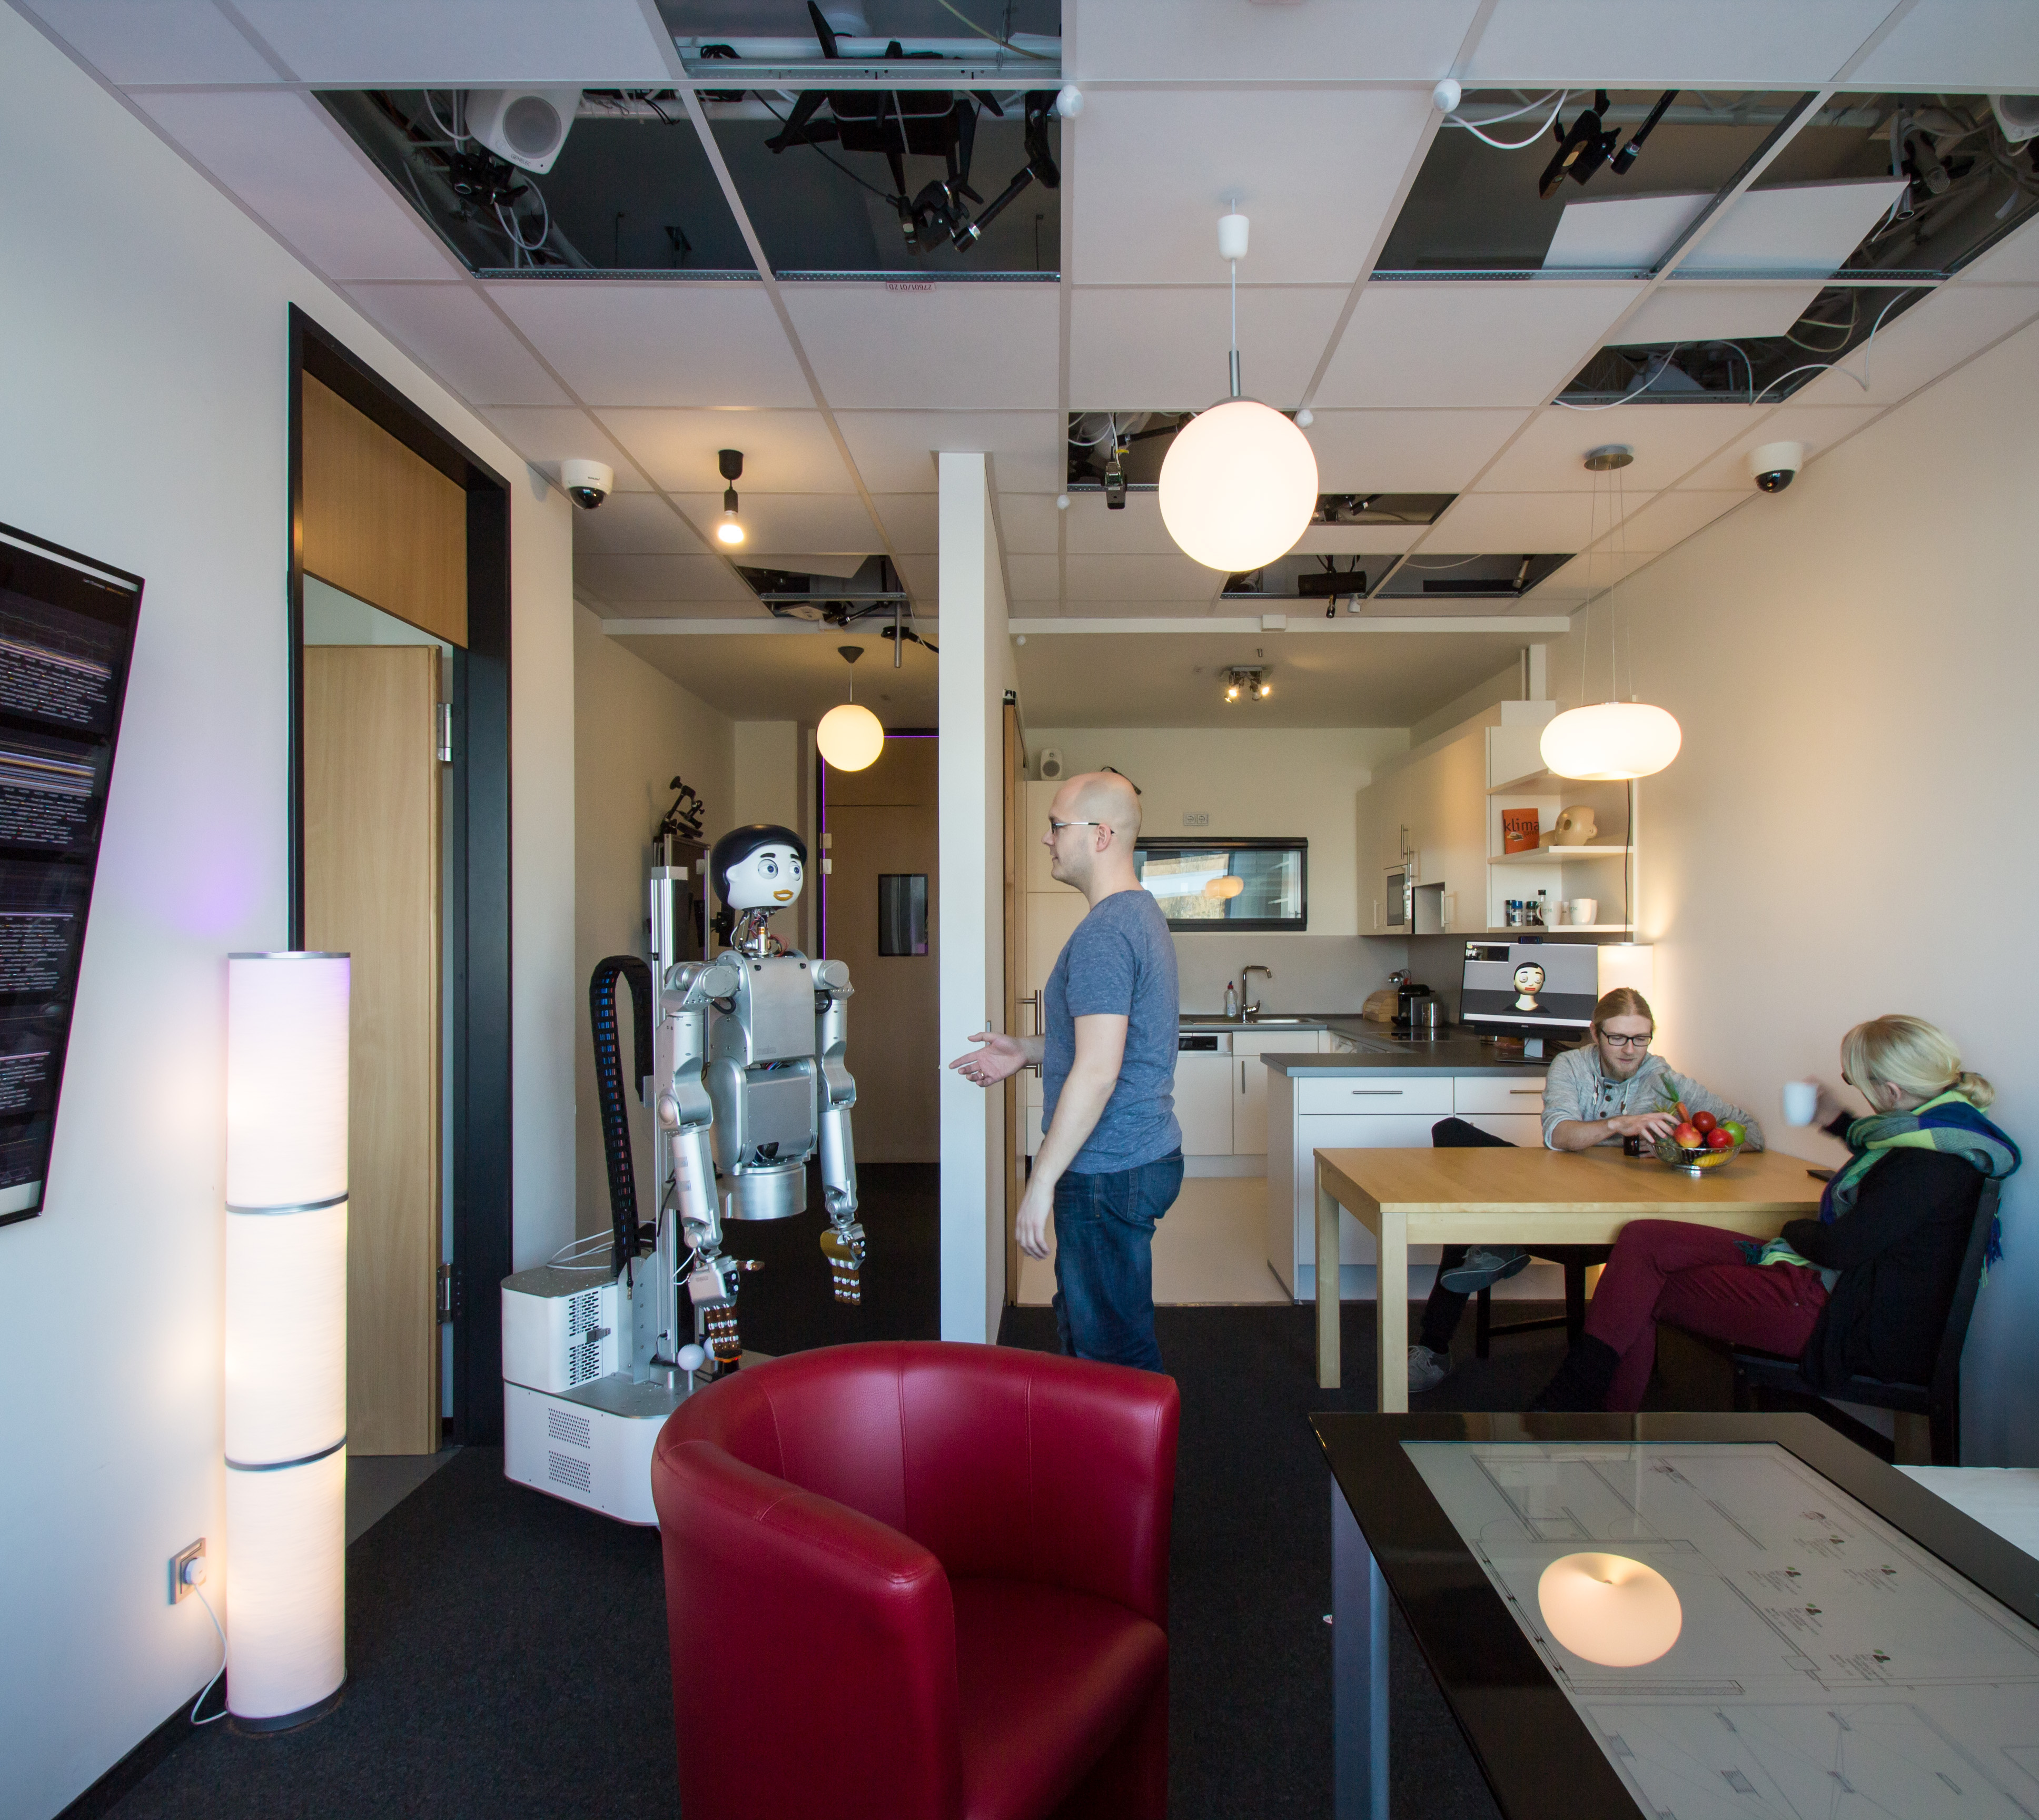
\includegraphics[trim={4cm 5cm 0cm 10cm},clip]{csra-windowshot}
        }
      };}
      \action<1->{\node (b) at (.5\textwidth+10,0)
      {
        \resizebox{.5\textwidth}{!}{%
          \includegraphics[trim={8cm 6cm 5cm 0},clip]{generated/elevator.jpg}
        }
      };}
    \end{tikzpicture}
  }
  \vspace{-10pt}\\
  \onslide<2->{\emph{
    Use the \textcolor<3->{myblue}{perceptive abilities} of the smart environment to recognize the \textcolor<4->{myblue}{conversational state} and expectations of inhabitants towards \textcolor<5->{myblue}{artificial agents}.
  }}
  \pnote{
    45-40 - csra full of interactive entities influences behaviour of inhabitants \\
    we do not want it to get awkward\\
    agents behave according to expectations\\
    need to know these expectations \\
    to approach this problem i formulate a goal (click)\\
  }
\end{frame}
\begin{frame}{Research Questions}
    \emph{\goalshort}
    \centering\\
    \vspace{10pt}
    \resizebox{1.\textwidth}{!}{%
        \footnotesize
        \begin{tikzpicture}
        \action<2->{\node (a) at (0,0)
        {
          \resizebox{.25\textwidth}{!}{%
            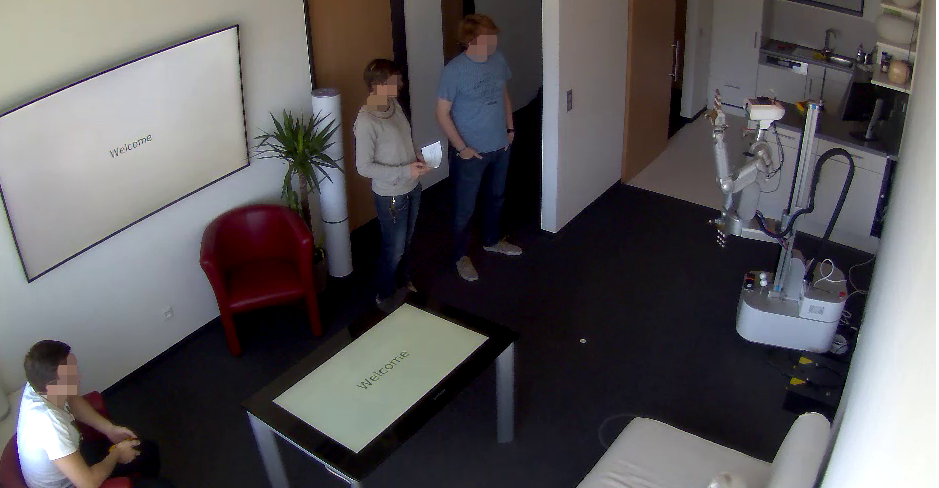
\includegraphics[trim={8cm 0 2cm 0},clip]{study-addressee-vp57}
          }
        };}
        \action<2->{\node[align=center, anchor=north, text width=.25\textwidth] (at) at (0, -.11\textwidth) {
        \textbf{RQ1 \scriptsize Addressing Behaviour}\\
          \vspace{5pt}
          Distinct \\ Addressed Entities
          };}
        \action<3->{\node (b) at (.25\textwidth+10,0)
        {
          \resizebox{.25\textwidth}{!}{%
            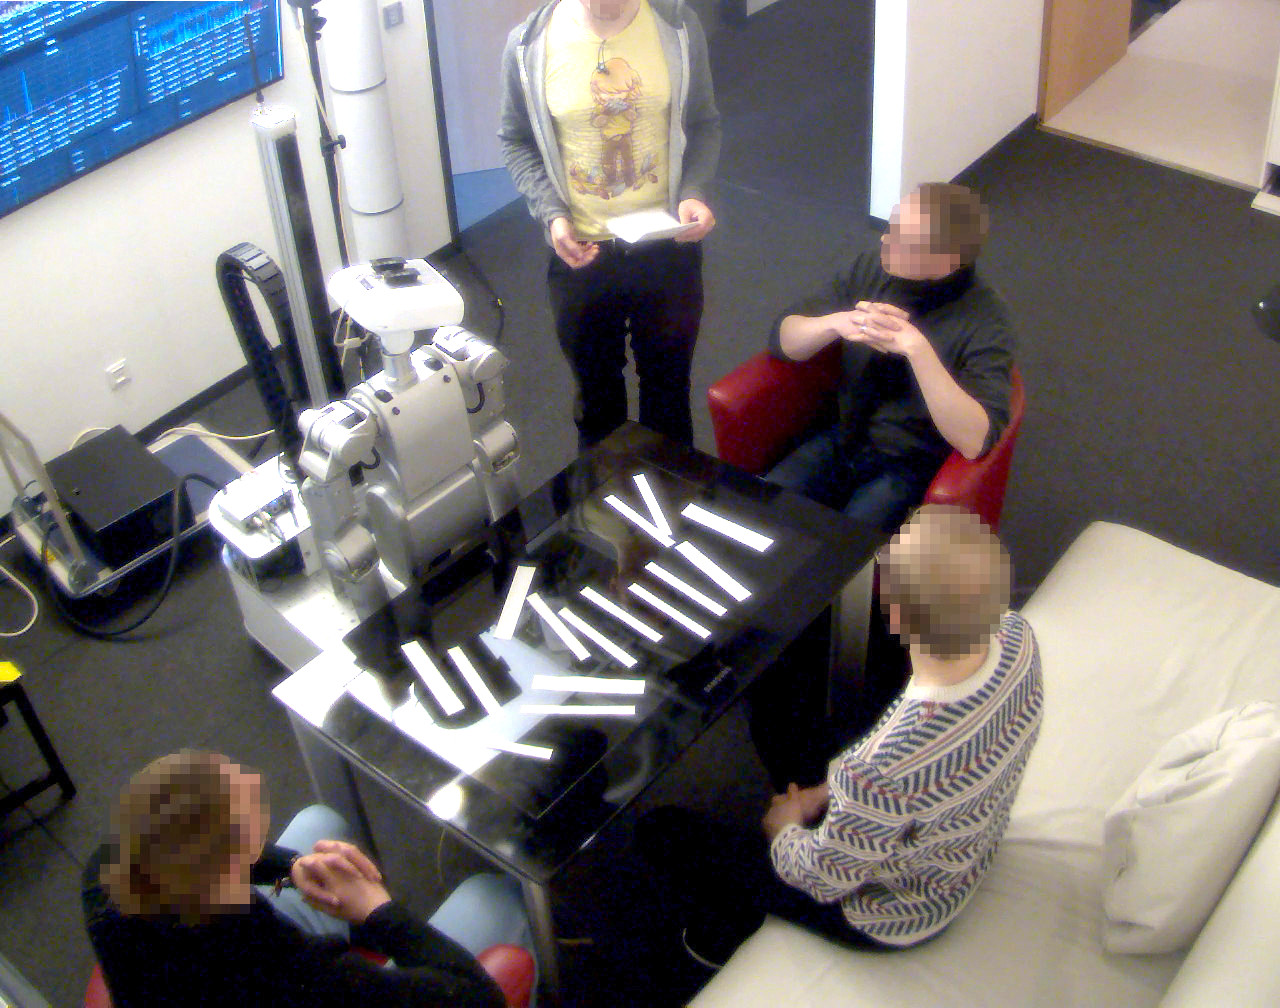
\includegraphics[trim={0 0 0 2cm},clip]{addressee-meka-intro}
          }
        };}
        \action<3->{\node[align=center, anchor=north, text width=.25\textwidth] (bt) at (.25\textwidth+10, -.11\textwidth) {
          \textbf{RQ2 \scriptsize Addressee Recognition}\\
          \vspace{5pt}
          React \\ to Addressing
          };}
        \action<4->{\node (c) at (.5\textwidth+20,0)
        {
          \resizebox{.25\textwidth}{!}{%
            \input{generated/conversational_group_defence.pdf_tex}
          }
        };}
        \action<4->{\node[align=center, anchor=north, text width=.25\textwidth] (ct) at (.5\textwidth+20, -.11\textwidth) {
          \textbf{RQ3 \scriptsize Conversational Group}\\
          \vspace{5pt}
          Participate \\ in Interaction
          };}
        \action<5->{\node (d) at (.75\textwidth+30,0)
        {
          \resizebox{.25\textwidth}{!}{%
            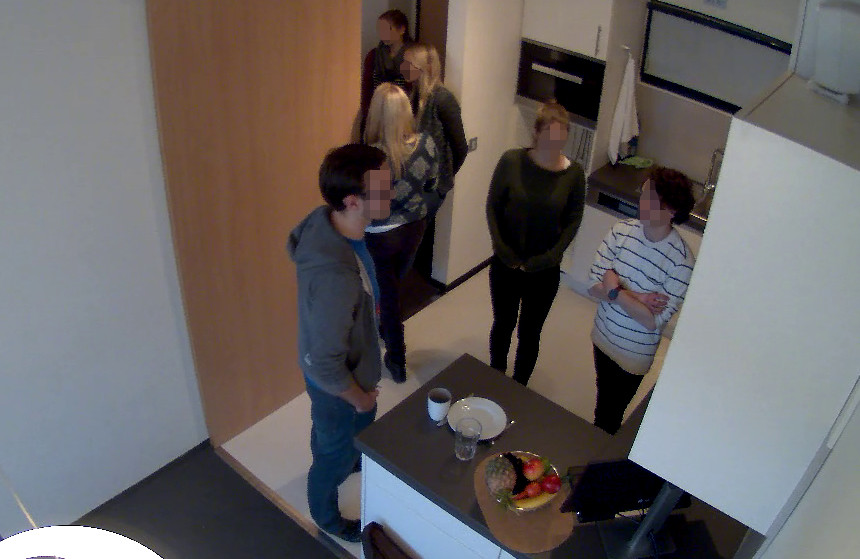
\includegraphics[trim={4.1cm 0 0 0},clip]{conversational_group}
          }
        };}
        \action<5->{\node[align=center, anchor=north, text width=.25\textwidth] (dt) at (.75\textwidth+30, -.11\textwidth) {
          \textbf{RQ4 \scriptsize Conversational Roles}\\
          \vspace{5pt}
          Repair \\ Interaction
        };}
\end{tikzpicture}
      }
    \pnote{
      45-40-to approach this goal i investigate 4 research questions\\
      }
\end{frame}

